\documentclass[12pt,twoside]{article}
\usepackage{jmlda}
%автомат

\title
    [HOG дескриптор для сверточной нейронной сети в задаче детектирования пешеходов] % Краткое название; не нужно, если полное название влезает в~колонтитул
	{Использование HOG дескриптора для сверточной нейронной сети в задаче детектирования пешеходов}
\author
    [Томинин~В.\,Д., Томинин~Я.\,Д., Демидова~Ю.\,О., Дудоров~Н.\,А., Ерлыгин~Л.\,О.] % список авторов для колонтитула; не нужен, если основной список влезает в колонтитул
    {Томинин~В.\,Д., Томинин~Я.\,Д., Демидова~Ю.\,О., Дудоров~Н.\,А., Ерлыгин~Л.\,О., Гнеушев~А.\,Н.} % основной список авторов, выводимый в оглавление
    [Томинин$^1$~В.\,Д., Томинин$^1$~Я.\,Д., Демидова$^1$~Ю.\,О., Дудоров$^1$~Н.\,А., Ерлыгин$^1$~Л.\,О., Гнеушев$^{1,2}$~А.\,Н.] % список авторов, выводимый в заголовок; не нужен, если он не отличается от основного
\thanks
    {Работа выполнена при финансовой поддержке РФФИ, проект \No\,00-00-00000.
   Научный руководитель: Матвеев~И.\,А. 
   Задачу поставил и консультировал: Гнеушев~А.\,Н.}
\email
    {tominin.vd@phystech.edu, tominin.yad@phystech.edu, demidova.ua@phystech.edu, zoom\_ccss@mail.ru, erlygin.la@phystech.edu, gneushev@ccas.ru}
\organization
    {$^1$Московский физико-технический институт, Россия, г. Долгопрудный, Институтский пер., 9\par
     $^2$ФИЦ <<Информатика и управление>> РАН, Россия, г. Москва, ул. Вавилова, 44/2}
\abstract
   {Рассматривается подход обобщения алгоритма HOG (Histograms of Oriented Gradients) для детектирования пешеходов 
   на изображении путем замены линейного бинарного классификатора SVM на сверточную нейронную сеть небольшой глубины. 
   Для возможности применения входных сверточных слоев нейросети в пространстве интегральных признаков в статье предлагается 
   преобразовать интегральный вектор HOG дескриптора в трехмерный тензор, имеющий две пространственные и одну спектральную 
   размерности, в соответствии с его внутренней блочной структурой. Учет локальной структуры HOG дескриптора позволяет 
   выделять дополнительные локальные признаки первыми сверточными слоями нейросети с целью оптимизации пространства HOG признаков 
   для классифицирующего слоя. В статье исследуются простые сверточные архитектуры нейросети, проведены вычислительных эксперименты 
   и представлены результаты сравнения работы базового алгоритма HOG-SVM и предлагаемых обобщений HOG-DNN и HOG-CNN на базах 
   изображений пешеходов INRIA и Cityscapes. 
   
\bigskip
\textbf{Ключевые слова}: \emph {HOG, CNN, гистограмм ориентированных градиентов, сверточные нейросети, детектирование пешехода}.}
\titleEng
    {Neural convolutional network based on HOG features for pedestrian detection}
\authorEng
    {Tominin$^1$~V.\,D., Tominin$^1$~Y.\,D., Demidova$^1$~U.\,O., Dudorov$^1$~N.\,A., Erlygin$^1$~L.\,A., Gneushev$^{1,2}$~A.\,N.}
\organizationEng
    {$^1$Moscow Institute of Physics and Technology, 9 Institutskiy per., Dolgoprudny, Moscow, Russia\par
	$^2$Federal Research Center ``Computer Science and Control'' of RAS, 44/2 Vavilova Str., Moscow, Russia}
\abstractEng
    {The approach of generalizing of HOG algorithm (Histograms of Oriented Gradients) for pedestrian detection on an image by replacing the linear binary classifier SVM with a convolutional neural network of shallow depth is considered. In order to use the imput convolutional layers of the neural network in the space of integral features, in this paper it is proposed to convert the integral vector of the HOG escriptor into a three-dimensional tensor having two spatial and one spectral dimensions according its internal block structures. The local structure of the HOG descriptor allows to select additional local features by the first convolutional layers of the neural network  to optimize the space of HOG features for the classifying layer. In the paper simple convolutional neural network architectures are studied, computational experiments are conducted and the results of the comparison of the basic HOG-SVM algorithm and the proposed generalizations of HOG-DNN and HOG-CNN on the INRIA and Cityscapes pedestrian databases are presented.
    	

    \bigskip
    \textbf{Keywords}: \emph{HOG, CNN, Histograms of Oriented Gradients, convolutional network, pedestrian detection}.}
\begin{document}
\maketitle
%\linenumbers
\section{Введение}
Автоматическое детектирование и распознавание объектов на изображениях является одной из основных задач компьютерного зрения. 
Задача локализации человека на видеоизображениях широко востребована в таких областях, как мониторинг и анализ дорожных ситуаций, обнаружение дорожно-транспортных происшествий, контроль за соблюдением правил дорожного движения, системы безопасности и следящие системы, беспилотные автомобили, робототехника, системы помощи водителю.

Основные сложности обнаружения человека на изображении связаны с несколькими причинами: изменение структуры изображения вследствие движения человека, неравномерная освещенность изображения, большая вариабельность изображений человека из-за разных ракурсов (поз, размеров, углов поворота), частичные перекрытия фигуры человека другими объектами.

Как правило, задача детектирования объекта разделяется на две подзадачи: выделение характерных свойств изображения объекта и бинарная классификация (рис. \ref{fg:TypicalImg}). Характерные свойства изображения объекта - это набор признаков, приближенно описывающий интересующий объект. Выбранный набор признаков является важнейшим фактором, влияющим на качество классификации и ее устойчивость. Чем лучше признаки обладают разделительной способностью (возможно, сложнее устроены), тем проще устроено признаковое пространство, и классификатор может иметь простой вид. Наоборот, чем менее уникальны признаки (но проще по структуре), тем сложнее устроено признаковое пространство и требуется более сложный классификатор для его успешного разделения. Наиболее эффективным в настоящее время является подход, объединяющий оба этап анализа изображения: одновременное выделение множества  признаков и их классификация многослойными сверточными нейронными сетями (CNN), в которых процедура выделения признаков осуществляется в начальных слоях, структура признаков формируется автоматически в процессе его обучения и определяется моделью и архитектурой сети. Чем больше признаков необходимо использовать для характеристики целевых объектов, тем больше параметров требуется для задания модели сети, тем она вычислительно сложнее и требует больше вычислительных ресурсов и объема обучающей выборки изображений. Это связано с тем, что в CNN признаковая модель объекта формируется на основе только той информации, которая содержится в обучающей базе и общих регуляризационных ограничениях. Привлекая априорную, более детальную экспертную информацию о характере конкретного класса объектов на изображении для построения модели пространства признаков, можно уменьшить количество параметров нейросети, ее вычислительную сложность и потребность в большом  объеме обучающей выборки.

\begin{figure}[h]
	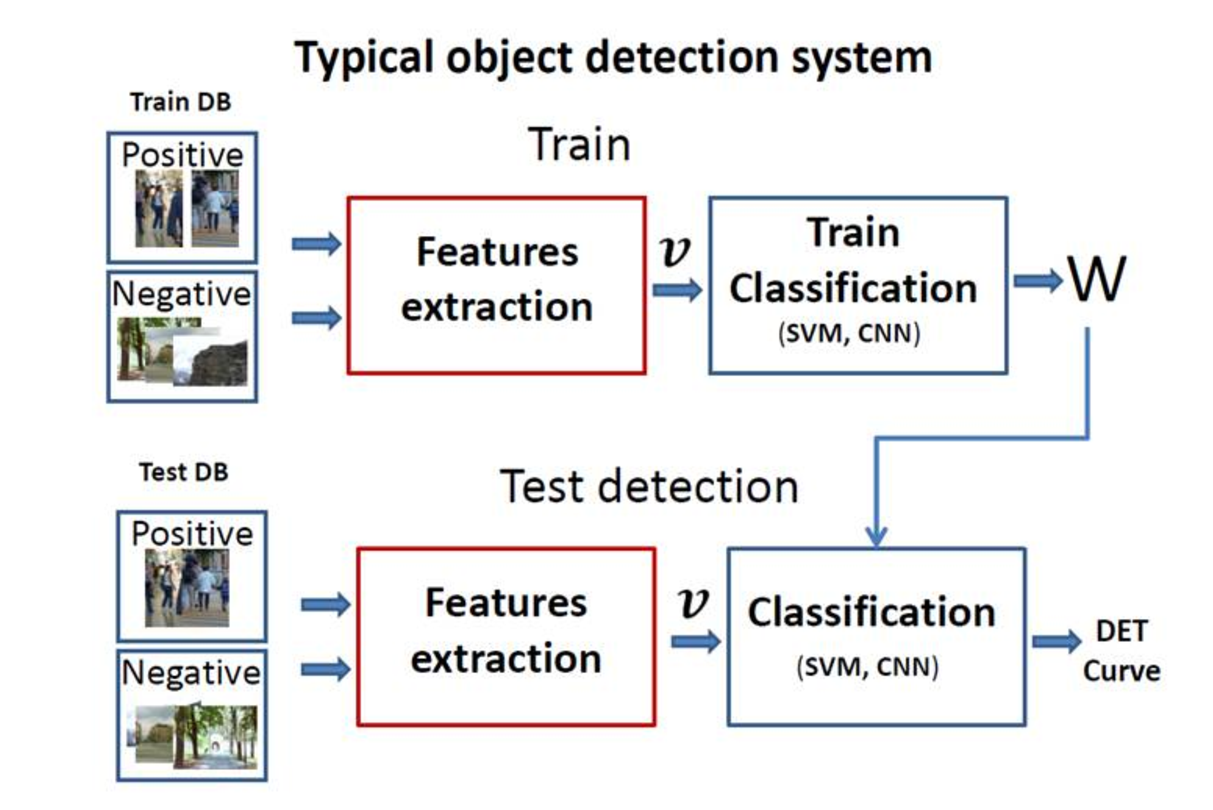
\includegraphics[width=\linewidth]{fig1}
	\caption{Типичная система детектирования объектов. }
	\label{fg:TypicalImg}
\end{figure}


Множество признаков, которые используются для раcпознавания объекта, определяются его характерной структурой на изображении. Изображение человека может быть представлено совокупностью контуров, силуэтов частей тела, которые являются контурными признаками и представляются на изображении как максимальные перепады значений яркости \cite{Gneushev03}. Эффективный алгоритм детектирования пешеходов, основанный на градиентах яркости изображения и учитывающий совокупность контурных признаков предложен в методе HOG~\cite{dalaltriggs2005} и подходах, которые его развивают~\cite{dpm, Samsonov17}. HOG-дескриптор обладает рядом преимуществ, он вычислительно
эффективен, показывает лучшие в своем классе результаты, однако для детектирования используется линейный классификатор SVM (Support Vector Machine), который предполагает линейную разделимость пространства признаков. Использование нелинейного классификатора может уменьшить ошибки детектирования особенно в сложных случаях с частичным перекрытием объектов, большой вариабельностью ракурса, в линейно неразделимом пространстве признаков. Таким образом, использование несложной сверточной нейронной сети в качестве нелинейного классификатора для пространства HOG дескрипторов с одной стороны позволяет задействовать все современные преимущества CNN, с другой стороны минимизировать сложность и вычислительную сложность детектора пешеходов в целом.

Обычно, для задачи классификации в интегральных признаковых пространствах используются полносвязные нейронные сети (DNN), так как в интегральных дескрипторах-векторах отсутствует локальная связность их компонент. Однако HOG дескриптор имеет внутреннюю блочную структуру по построению, и каждый определенный участок интегрального вектора HOG дескриптора является локальным дескриптором блока изображения, локальной области. В данной работе предлагается использовать эту информацию и преобразовать интегральный вектор HOG дескриптора в трехмерный тензор, имеющий две пространственные и одну спектральную размерности, и сохраняющий внутреннюю блочную структуру дескриптора. Данный подход позволяет использовать сверточные входные слои нейросети и, следовательно, использовать глубокое обучение на HOG пространстве. Учет локальной структуры HOG дескриптора позволяет выделять дополнительные локальные признаки первыми слоями нейросети с целью оптимизации пространства HOG признаков для финального классифицирующего слоя.

\section{Существующие подходы}
Исследователи используют несколько подходов к решению задачи обнаружения объектов на изображениях, но мы упоминаем здесь лишь несколько: оригинальный метод HOG, на котором основана данная работа, а также несколько подходов, которые его развивают. 

Наш подход основан на алгоритме HOG~\cite{dalaltriggs2005} для детектирования пешеходов, напоминающий гистограммы направления края, дескрипторы SIFT и контексты формы, но расчет ведется на плотной сетке равномерно расположенных ячеек и производится нормализация перекрывающегося локального контраста. Для бинарной классификации используется SVM~\cite{Vorontsov}. Установлено, что для получения хороших результатов необходимо относительно грубое разбиение пространства, точное вычисление направлений и сильная локальная нормализация контраста в перекрывающихся блоках. Интегральный вектор HOG дескриптора превосходит другие рассматриваемые дескрипторы. Новый подход обеспечивает почти идеальное разделение исходной базы данных пешеходов MIT, поэтому была создана новая, более сложная база данных INRIA~\cite{inria}.

Исследователи предлагают несколько подходов развития метода HOG. В статье~\cite{Samsonov17} предлагается использовать аккумуляторное пространство Хафа для обобщения HOG дескриптора путем получения гистограмм аккумуляторного пространства Хафа (Hough Accumulator Histograms, HAH). Пространство Хафа строится на основе лучевого поперечного преобразования Радона градиентного поля изображения. Использование проекций в аккумуляторном пространстве Хафа позволяет учитывать не только локальное распределение ориентаций контурных признаков, но и их положение, что дает дополнительную информацию. На основе данного подхода описаны несколько дескрипторов, которые превосходят HOG дескриптор~\cite{dalaltriggs2005} по качеству детектирования. Данные методы протестированы с помощью линейного SVM  на базе изображений пешеходов INRIA. 
% обзор литературы

\section{Постановка задачи}
Рассмотрим структуру интегрального вектора признаков $\vec{g}(f) = (g_{1},\dots , g_{n})^{\mathrm{T}}$ HOG дескриптора \cite{dalaltriggs2005} из признакового пространства $G$ для входного изображения $f$, где $n$~--- размерность пространства признаков. В соответствии со схемой
HOG, изображение $f(x,y)$, где $x$, $y$~--– координаты точки изображения размером $X\times Y$, разбивается на смежные области~--– квадратные ячейки размером $K\times K$ пикселей, $I=X/K$ ячеек по горизонтали и $J=Y/K$ ячеек по вертикали. 
В каждой ячейке $(i,j)$, где $i$, $j$~--- индексы ячейки по вертикали 	и горизонтали соответственно, выделяются локальные признаки, которые определяются дескриптором ячейки~--- вектором $\vec{u}_{i,j} = (u_1, \dots , u_l)^{\mathrm{T}}$, где $l$~---	размерность вектора. Четыре смежные ячейки объединяются в пересекающиеся блоки. Таким образом, каждый блок содержит $2K \times 2K$ пикселей и имеет общие ячейки с соседними блоками. Дескриптор блока определяется объединением дескрипторов собственных ячеек, вектором $\vec{v}_{i,j} = \vec{u}_{i,j}\cup\vec{u}_{i+1,j}\cup\vec{u}_{i,j+1}
	\cup\vec{u}_{i+1,j+1},$ где $i$,$j$~--- индексы блока.
	Общее количество блоков~--- $(I-1)(J-1)$. Под операцией
	объединения $\cup$ двух векторов $\vec{u}_{1}$ и $\vec{u}_{2}$
	c размерностью $l_{1}$ и $l_{2}$ соответственно будем понимать результирующий вектор из пространства размерности $l_{1}+l_{2}$, первые $l_{1}$ компонент которого являются компонентами вектора первого аргумента, последние $l_{2}$ ~--- компонентами вектора второго аргумента.
	
	 Дескриптор блока нормируется с помощью одной из двух норм:
		 $L_2$ нормы
\begin{equation*}
	\vec{\tilde{v}} = N_{L_{2}}(\vec{v}) =  \frac{\vec{v}}{\sqrt{\Vert \vec{v} \Vert_{2}^{2} + \epsilon^{2}}}
	\label{eq:L2}
\end{equation*}
либо $L_2$--hys нормы \cite{dalaltriggs2005}
\begin{equation*}
	\vec{\tilde{v}} = N_{L_{2}-\mathrm{hys}}(\vec{v}) =  N_{L_{2}}
	\left(\min(N_{L_{2}}(\vec{v}),h)\right),
	\label{eq:L2-hys}
\end{equation*}
где операция $\min$ применяется покомпонентно к вектору первого
аргумента; $h$~--- пороговое значение, которое используется для
ограничения значений компонент вектора в~операции $\min$. В данной работе, как и в работе \cite{dalaltriggs2005}, в качестве порогового значения используется $h=0{,}2$.


Интегральный дескриптор определяется объединением всех
блочных дескрипторов, т.\,е.\ вектором
\begin{equation}
\vec {g}=\bigcup_j^{J-1}{\bigcup_i^{I-1}{\vec{\tilde{v}}_{i,j}}}\,.
\end{equation}
Интегральные дескрипторы $\vec{g}$ множества изображений формируют
признаковое пространство $G$. 

В работе ставится задача преобразования признакового векторного пространства $G$ в трехмерное тензорное пространство с размерностью ${2(I-1)}\times{2(J-1})\times{l}$, восстанавливающее пространственную смежность дескрипторов ячеек $\vec{u}$ из блоков $\vec{v}$ вектора $\vec{g}$. Используя тензорное представление вектора $\vec{g}$ реализовать сверточную нейронную сети одной из известных архитектур для решения задачи разбиения этого пространства
на два непересекающихся класса: первый характеризует пешеходов; второй~--- фон, не содержащий пешехода. 

Множество весов и параметров нейросетевого классификатора находятся из процедуры обучения по специально подготовленной 
обучающей выборке из базы изображений INRIA, CityScapes \cite{inria} содержащие два подмножества изображений: 
с~положительными примерами, содержащими пешеходов, и отрицательными примерами, содержащими фон.

	Критерием качества классификации  на специально
	подготовленной тестовой выборке из базы изображений INRIA \cite{inria} и CityScapes
	будем считать отношение $\mathrm{MR} = \mathrm{FN}/(\mathrm{TP}+\mathrm{FN})$~---
	доля неверно отвергнутых классификатором изображений ($\mathrm{Miss\ Rate}$),
	к $\mathrm{FPPW} = \mathrm{FP}/(\mathrm{TN}+\mathrm{FP})$~---
	доля неверно принятых изображений ($\mathrm{False\ Positive\ Per\
	Window}$), где $\mathrm{FN}$~--- количество неверно отвергнутых
	классификатором положительных примеров; $\mathrm{TP}$~---
	количество верно классифицированных положительных примеров;
	$\mathrm{TN}$~--- количество верно классифицированных отрицательных
	примеров; $\mathrm{FP}$~--- количество неверно классифицированных отрицательных примеров.


\section{Тензорное представление HOG дескриптора для CNN}
Полученный интегральный дескриптор $\textbf{g}$(Рис.~\ref{ris:1}) является объединением всех блочных дейскрипторов. Признаковое пространство G имеет размерность ${2(I-1)}{2(J-1}){l}$. Для востановления пространственной смежности ячеек нужно перейти в новое трехмерное тензорное пространство с размерностью  ${2(I-1)}\times{2(J-1})\times{l}$. \\

\begin{center}
	
	\begin{figure}[H]
		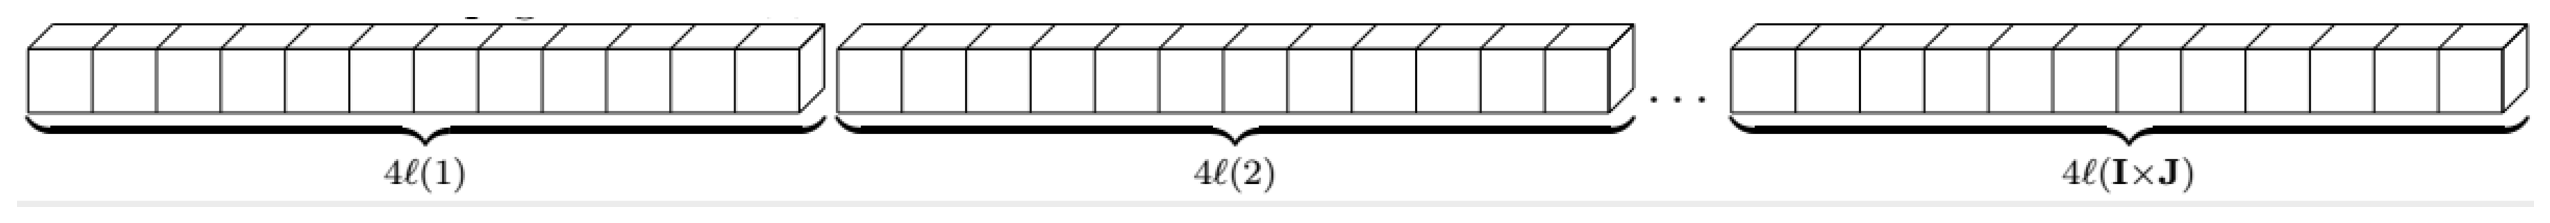
\includegraphics[width=\linewidth]{1}
		\caption{Изначально вектор g имеет вид}
		\label{ris:1}
	\end{figure}
\end{center}
Далее проводится операция с каждым вектором размерности $4 \ell$. Рассмотрим произвольный вектор блока $\vec{v}_{i,j} = \vec{u}_{i,j}\cup\vec{u}_{i+1,j}\cup\vec{u}_{i,j+1}
\cup\vec{u}_{i+1,j+1},$ где $i$,$j$~--- индексы блока; $\vec{u}_{ij}$-вектор ячейки (i,j). 
Состаим тензор $\textbf{Z}_{ij}$ 
размерности $2\times 2 \times \ell$, 
причем $Z_{ij}[0][0]=\vec{u}_{i,j}$, $Z_{ij}[0][1]=\vec{u}_{i,j+1}$, $Z_{ij}[1][0]=\vec{u}_{i+1,j}$, $Z_{ij}[1][1]=\vec{u}_{i+1,j+1}$.(Рис.~\ref{ris:2})
\begin{center}
	\begin{figure}[H]
		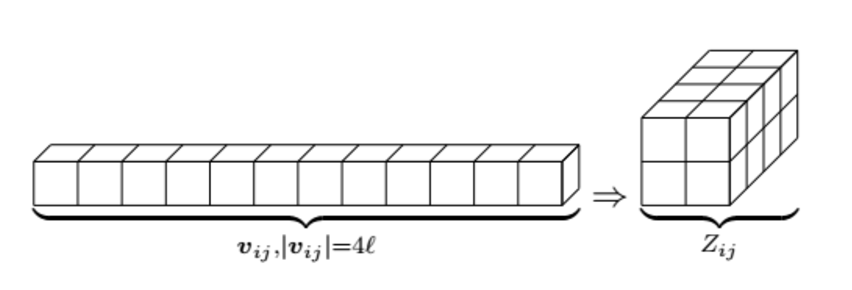
\includegraphics[width=0.6\linewidth]{2}
		\caption{Изменение размерности вектора длины $4 \ell$ }
		\label{ris:2}
	\end{figure}
\end{center}
Для каждого $j=1\div \textbf{J}-1$ составим тензор $\textbf{W}_j=\textbf{Z}_{1j}\cdot\textbf{Z}_{2j}\cdot ... \cdot \textbf{Z}_{(I-1)j} $(Рис.~\ref{ris:3}), здесь под операцией $\textbf{Z}_{ij} \cdot \textbf{Z}_{we}$ подразумевается покомпонентное объединение векторов $\textbf{Z}_{ij}[:][k][q] \cup \textbf{Z}_{we}[:][k][q]$ , где $k=1\div 2; q=1\div \ell$
\begin{center}
	\begin{figure}[H]
		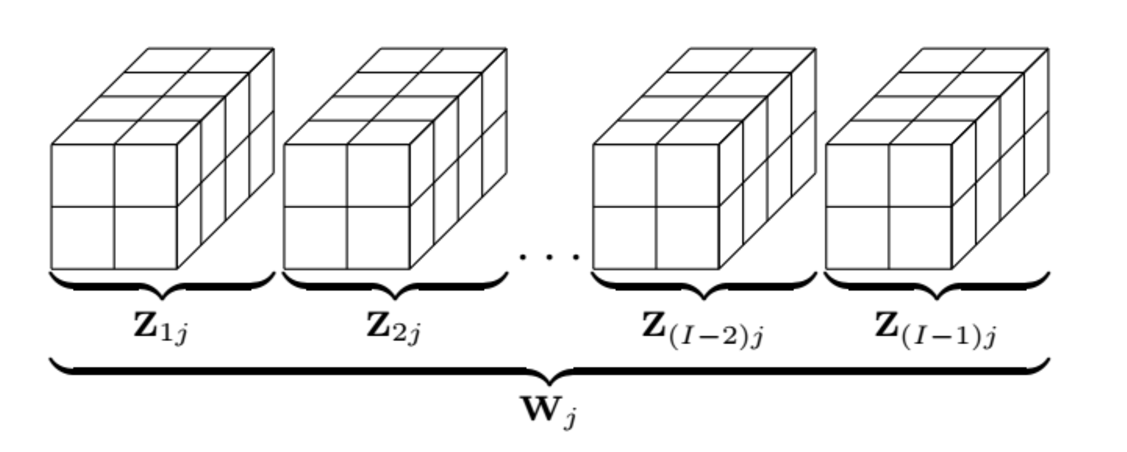
\includegraphics[width=0.7\linewidth]{3}
		\caption{Получение тензора $\textbf{W}$ размерности $2\textbf{I}\times 2 \times \ell$ }
		\label{ris:3}
	\end{figure}
\end{center}
Далее получим тензор $\textbf{R}$, который будет соответстовать трехмерному тензорному пространству с размерностью  
${2(I-1)}\times {2(J-1})\times {l}$ по формуле 
$\textbf{R}=\textbf{W}_1 \circ \textbf{W}_2 \circ ... \circ \textbf{W}_{J-1}$
(Рис.~\ref{ris:4}), где под операцией $\textbf{W}_j \circ \textbf{W}_i$ подразумевается покомпонентное объединение векторов $\textbf{W}_{j}[k][:][q] \cup \textbf{W}_i[k][:][q]$ ,  $k=1\div 2(\textbf{I}-1); q=1\div \ell$.
\begin{center}
	\begin{figure}[H]
		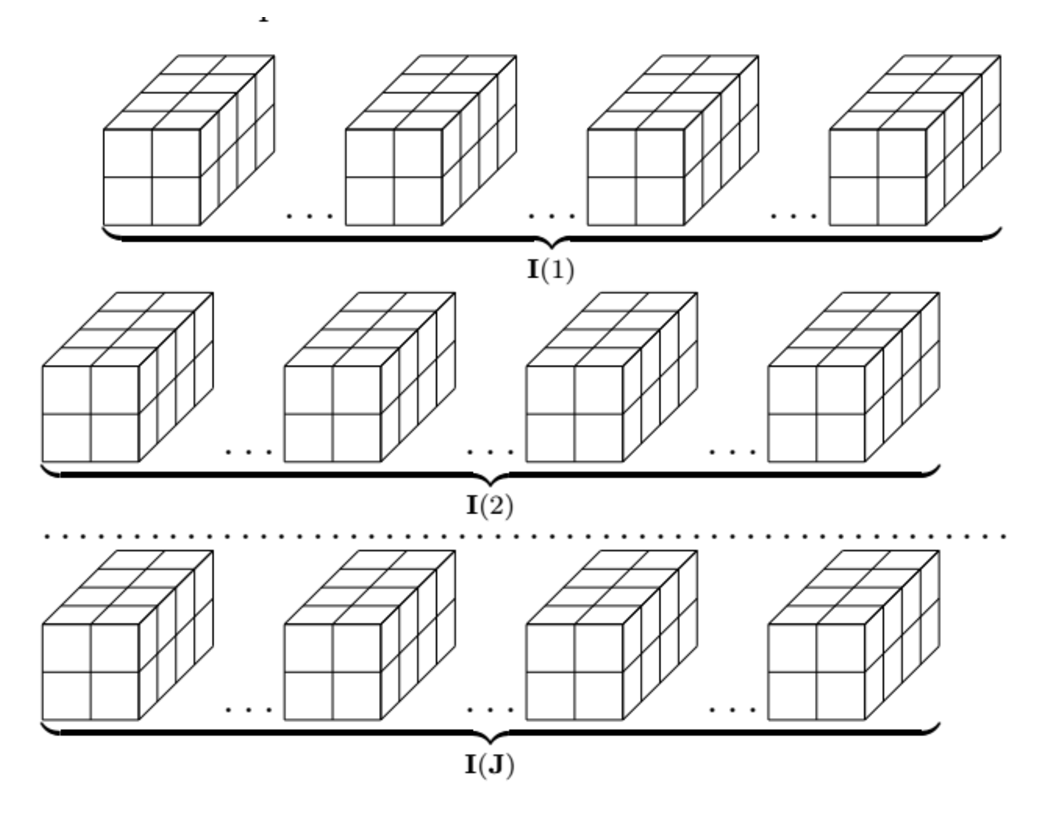
\includegraphics[width=0.6\linewidth]{4}
		\caption{Трехмерное тензорное пространство $\textbf{R}$с размерностью  ${2(I-1)}\times {2(J-1})\times {l}$}
		\label{ris:4}
	\end{figure}
	
\end{center}
Полученный тензор $\textbf{R}$, имеющий размерность  ${2(I-1)}\times {2(J-1})\times {l}$, будет подаваться в нейронную сеть. 


\section{Результаты вычислительных экспериментов}
Целью вычислительных экспериментов является проверка работы предлагаемого в статье метода на реальных данных, а также сравнение его качества детектирования и времени работы с аналогичными показателями HOG дескриптора.
В качестве обучающей выборки была использована база изображений INRIA. В базу входит 2478 изображений пешеходов размером $96 \times 160$ пикселей.
Из каждого положительного изображения выбирается окно размером 64 пикселей, центр которого совпадает с центром изображения. Таким образом, 2478 изображений составляют положительную часть обучающей выборки.
Также база содержит 1218 изображений фона, из которых в отрицательную чать обучающей выборки выделяется 12180 окон размером 64 пикселей, центр окна определяется случайно.
Для обучения классификатора была использована библиотека OpenCV, классификатор обучался с помощью линейного метода SVM.

\begin{center}
	\begin{picture}(120,120)
	\put(-75,80){\framebox(300,15){Признаковое описание изображения}}
	\put(75,80){\vector(0,-1){12.5}}
	\put(-75,52.5){\framebox(300,15){Обучение модели}}
	\put(75,52.5){\vector(0,-1){12.5}}
	\put(-75,25){\framebox(300,15){Вычисление результатов модели на тестовой выборке}}
	\end{picture}
\end{center}


\begin{figure}[h]
	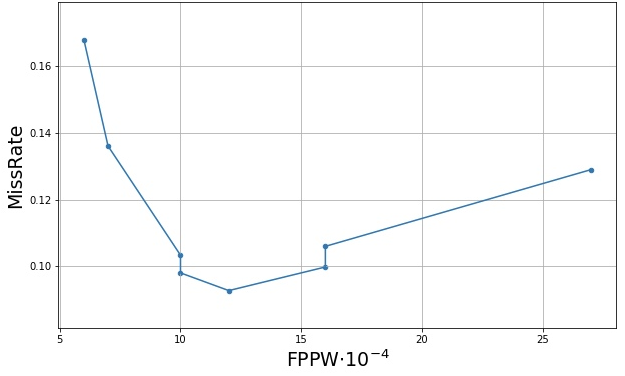
\includegraphics[width=0.8\linewidth]{detcurve}
	\caption{DET - кривая для HOG+SVM }
	%\label{fg:Example}
\end{figure}



\begin{center}
	\begin{tabular}{| l | l | l |}
		\hline
		{Метод} & {Miss Rate at $10^{-4}FPPW$, INRIA} & {Miss Rate at $10^{-4}FPPW$, CityScapes} \\ \hline
		{HOG-SVM} & {$0.12$} & {$-$} \\ \hline
		{HOG-DNN-2} & {$-$} & {$-$} \\ \hline
		{HOG-CNN-3} & {$-$} & {$-$} \\ \hline
	\end{tabular}
	\newline
\end{center}

\section{Заключение}
В работе представлен подход обобщения алгоритма HOG для детектирования пешеходов 
на изображении путем замены линейного бинарного классификатора SVM на сверточную нейронную сеть небольшой глубины.
Представлены результаты вычислительного эксперимента с использованием сверточной нейронной сети небольшой глубины и их сравнение с HOG-дескриптором по производительности. 
Учет локальной структуры HOG дескриптора позволяет выделять дополнительные локальные признаки первыми сверточными слоями нейросети с целью оптимизации пространства HOG признаков для классифицирующего слоя.
Основным недостатком предлагаемого подхода является довольно низкая производительность, вызванная оптимизацией весов нейронной сети на каждом шаге обучения. 

\bigskip
%\newpage
\maketitleSecondary
%\English

\bibliographystyle{unsrt}
\bibliography{jmlda-bib}

\begin{thebibliography}{99}
\bibitem{Gneushev03}
Gneushev, A.\,N., and A.\,B.~Murynin.	
2003. Adaptive gradient method for extracting contour features of
objects in images of real-world scenes.
\BibJournal{J.~Comput. Sys. Sci. Int.} 42(6):973--980.

\bibitem{Samsonov17}
Samsonov N.\,A., Gneushev, A.\,N.	
2017. Textural descriptor in the Hough accumulator space of the gradient field for detecting pedestrians.
\BibJournal{Machine Learning and Data Analysis} 3(3):203--215.


\bibitem{dalaltriggs2005}
Dalal,~N., and B.~Triggs. 2005.
 Histograms of oriented gradients for
human detection. \BibJournal{IEEE CVPR}. San Diego, CA.

\bibitem{dpm}
	{Felzenszwalb,~P.\,F., B.\,R.~Girshick, D.~McAllester,
	and D.~Ramanan}. 2010.
	Object detection with discriminatively trained part based models.
\BibJournal{IEEE T.~Patt. Anal.} 32(9):1627--1645.

\bibitem{sunwatanada2015}
	{Sun,~D., and J.~Watanada}, 2015.
	Detecting pedestrians and vehicles in traffic scene based on
	boosted HOG features and SVM.
\BibJournal{IEEE 9th  Symposium (International)
on Intelligent Signal Processing}.

\bibitem{inria}
	INRIA Person Dataset.
	Avalaible at: {\sf http://pascal.inrialpes.fr/data/human/}
	(accessed June~4, 2017).

\bibitem{opencv}
	Open Source Computer Vision Library.
	Avalaible at: {\sf http://opencv.org/releases.html}
	(accessed May 16, 2017).
	
\bibitem{Vorontsov}
	Vorontsov, K.\,V. 2007. Lectures on support vector machine.
	{\sf http://www.ccas.ru/voron/download/\linebreak SVM.pdf}
	(accessed June~25, 2017).

\end{thebibliography}

%\begin{thebibliography}{1}

%\bibitem{author09anyscience}
%    \BibAuthor{Author\;N.}
%    \BibTitle{Paper title}~//
%    \BibJournal{10-th Int'l. Conf. on Anyscience}, 2009.  Vol.\,11, No.\,1.  Pp.\,111--122.
%\bibitem{myHandbook}
%    \BibAuthor{Автор\;И.\,О.}
%    Название книги.
%    Город: Издательство, 2009. 314~с.
%\bibitem{author09first-word-of-the-title}
%    \BibAuthor{Автор\;И.\,О.}
%    \BibTitle{Название статьи}~//
%    \BibJournal{Название конференции или сборника},
%    Город:~Изд-во, 2009.  С.\,5--6.
%\bibitem{author-and-co2007}
%    \BibAuthor{Автор\;И.\,О., Соавтор\;И.\,О.}
%    \BibTitle{Название статьи}~//
%    \BibJournal{Название журнала}. 2007. Т.\,38, \No\,5. С.\,54--62.
%\bibitem{bibUsefulUrl}
%    \BibUrl{www.site.ru}~---
%    Название сайта.  2007.
%\bibitem{voron06latex}
%    \BibAuthor{Воронцов~К.\,В.}
%    \LaTeXe\ в~примерах.
%    2006.
%    \BibUrl{http://www.ccas.ru/voron/latex.html}.
%\bibitem{Lvovsky03}
%    \BibAuthor{Львовский~С.\,М.} Набор и вёрстка в пакете~\LaTeX.
%    3-е издание.
%    Москва:~МЦHМО, 2003.  448~с.
%\end{thebibliography}

% Решение Программного Комитета:
%\ACCEPTNOTE
%\AMENDNOTE
%\REJECTNOTE
\end{document}